\section{Phase reduction theory}

We first review the phase reduction theory for ordinary differential equations (ODEs) in this section.
The approach is basically composed of three steps:
(i) We first define the phase of an ODE having a stable periodic orbit,
(ii) then we derive the phase equation of a perturbed ODE,
and (iii) finally we make a simplification of the phase equation by using the method of averaging.
In the following, we briefly review these three steps, which follow the analysis procedure presented in \cite{kori2011}.

\subsection{Definition of phases}
We begin by considering an ordinary differential equation (ODE) of the form,
\begin{align}
  \frac{\diff x}{\diff t}=f(x),
  \label{eq:ode}
\end{align}
where $x\in\mathbb{R}^{d}$ is a $d$-dimensional vector representing a state and $f\colon\mathbb{R}^{d}\to\mathbb{R}^{d}$ is a smooth vector field.
We assume that this ODE has a stable periodic orbit $p(t)$ with a period $T$.

After sufficiently long time, the state $x(t)$ of the ODE (\ref{eq:ode}) approaches the periodic orbit.
We can define a \textbf{phase} on such a periodic orbit $p(t)$ as follows,
\begin{align}
  \phi(p(t))=\omega t,
\end{align}
where $\omega=2\pi/T$ is the angular velocity of the periodic orbit.
This phase can be seen as a filed over the input space $\mathbb{R}^{d}$,
but it is now only defined over the periodic orbit $p(t) \subset \mathbb{R}^{d}$.
We extend the definition of the phase to the whole input space $\mathbb{R}^{d}$.
It is mathematically proved that for an initial point $x_{0}$ with the orbit $x(t; x_{0})$\footnote{In the following, we denote $x(t;x_{0})$ by the solution of the ODE (\ref{eq:ode}) with the initial condition $x(0)=x_{0}$.},
we can find a phase $\phi_{0}$ with
\begin{align}
  \lim_{t\to\infty}\|x(t;x_{0})-p(\phi_{0}/\omega+t)\|=0,
  \label{eq:phase}
\end{align}
as long as $x_{0}$ resides in a basin of the periodic orbit $p(t)$.
Then we define the phase $\phi(x_{0})$ as $\phi_{0}$.
We note that the phase $\phi_{0}$ is uniquely determined up to a $2\pi$ modulus for every point $x_{0}$ in a basin.
A set $\{x\in\mathrm{basin} \mid \phi(x)=\phi_{0}\}$ is called an \textbf{isochron} for the phase $\phi_{0}$.
We demonstrate phase fields for several ODEs having a stable periodic orbit in Figure \ref{fig:isochronous_map}.

\begin{figure}[htbp]
  \centering
  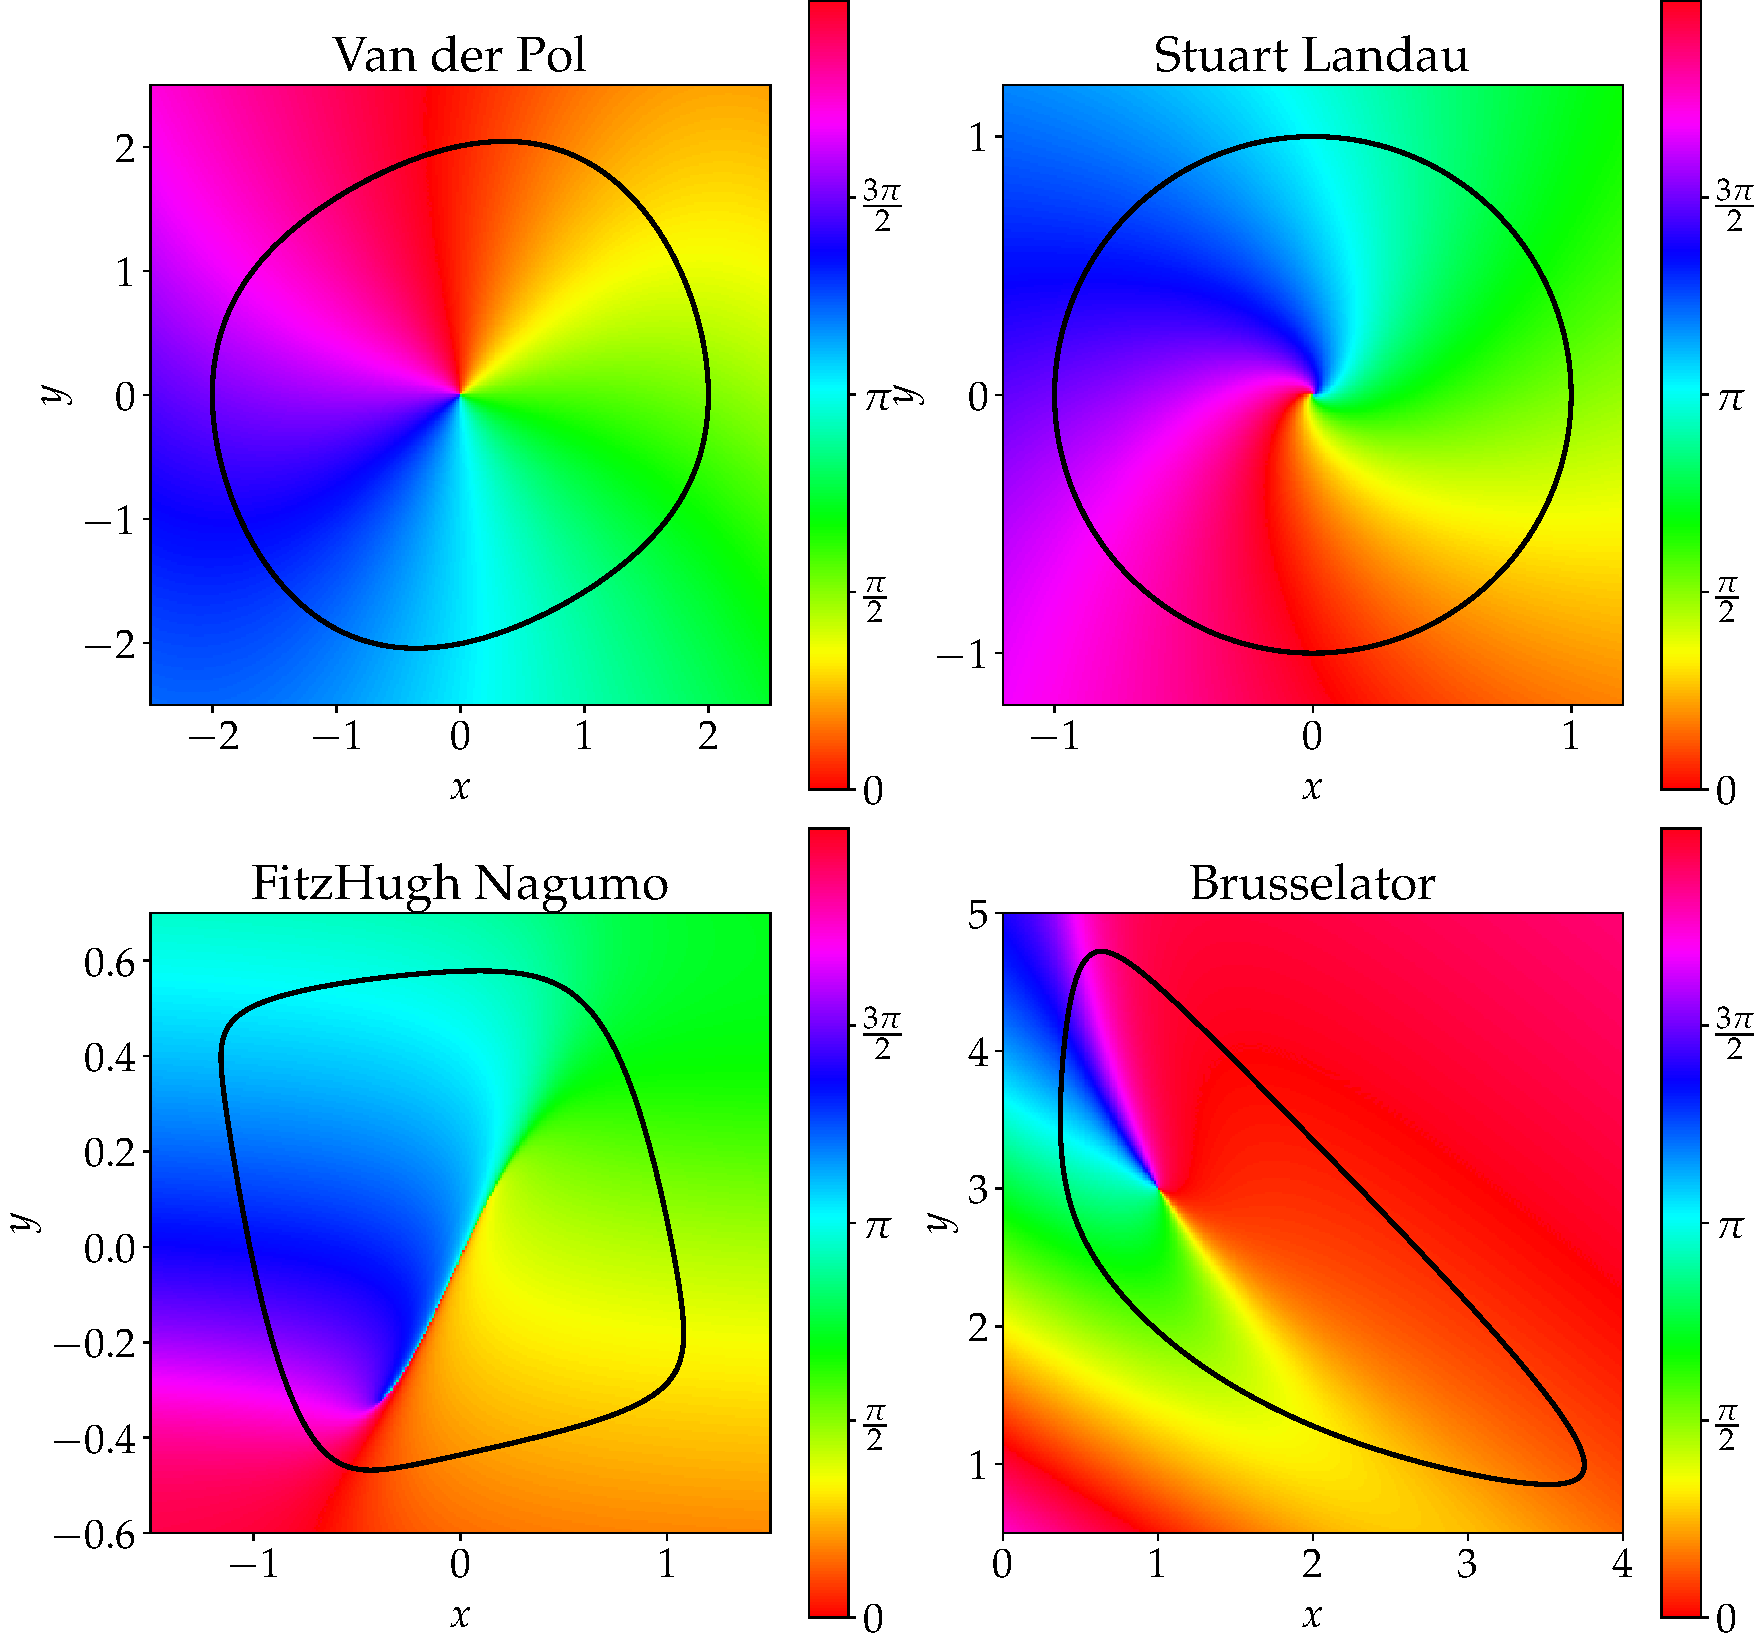
\includegraphics[width=0.7\textwidth]{figs/isochronous_map.pdf}
  \caption{The phase fields for the Van der Pol oscillator, the Stuart-Landau oscillator, the FitzHugh-Nagumo oscillator, and the Brusselator oscillator.
  The black lines denote periodic solutions.}
  \label{fig:isochronous_map}
\end{figure}

We note some properties of the phase field.
If $\phi(x_{0})=\phi_{0}$ for $x_{0}\in\mathbb{R}^{d}$,
then for a time shift $\phi(x(\Delta t;x_{0}))=\phi_{0}+\omega\Delta t$.
This can be seen from the property of the orbit $x(t;x(\Delta t; x_{0}))=x(t+\Delta t; x_{0})$ and the following calculation:
\begin{align}
\left\|x(t;x(\Delta t; x_{0}))-p\left(\frac{\phi_{0}+\omega\Delta t}{\omega}+t\right)\right\|
=\|x(t+\Delta t; x_{0})-p(\phi_{0}/\omega+(t+\Delta t))\|\to 0,
\end{align}
as $t\to\infty$.
Therefore the differentiation of the phase on the orbit over time is $\omega$, that is,
\begin{align}
  \frac{\diff\phi(x(t))}{\diff t}=\lim_{\Delta t\to 0}\frac{\phi(x(t+\Delta t))- \phi(x(t))}{\Delta t}=\omega.
  \label{eq:unperturbed-phase-diff}
\end{align}
Or, we can also write this as
\begin{align}
  \frac{\partial\phi}{\partial x}\frac{\diff x}{\diff t}=\frac{\partial\phi}{\partial x}f(x)=\omega,
  \label{eq:unperturbed-phase-diff-2}
\end{align}
by the use of the chain rule.
We can view this as a \textbf{phase equation} for an unperturbed ODE system~\eqref{eq:ode} (as opposed to the phase equation for a perturbed system, which we will discuss later).
In the following, we may simply write $\frac{\diff\phi}{\diff t}=\omega$ as if the phase itself is developing in time along the ODE~\eqref{eq:ode}.
Also, by taking $\Delta t=mT$ for integer $m$, we have
\begin{align}
  \phi(x(mT))\equiv\phi(x(0)) \bmod 2\pi.
\end{align}
Therefore $x(mT)$ resides in the same isochron as $x(0)$ for any $m\in\mathbb{Z}$.

\subsection{Phases for perturbed systems}
In the previous subsection, we have defined a phase field for a system with a stable periodic orbit,
and obtained the phase equation~\eqref{eq:unperturbed-phase-diff}.
Our next challenge is to find a perturbed version of the phase equation.

We set a perturbed ODE as follows,
\begin{align}
  \frac{\diff x}{\diff t}=f(x)+\varepsilon g(t,x),
  \label{eq:ode-perturbed}
\end{align}
where $g\colon\mathbb{R}\times\mathbb{R}^{d}\to\mathbb{R}^{d}$ is a perturbation function and $\varepsilon$ denotes its strength.
We assume that the perturbation function $g$ is sufficiently smooth as we need.
By substituting \eqref{eq:unperturbed-phase-diff-2} and \eqref{eq:ode-perturbed},
we have the phase equation for the perturbed system as
\begin{align}
  \frac{\diff\phi}{\diff t}=\frac{\partial\phi}{\partial x}\frac{\diff x}{\diff t}=\omega+\varepsilon\frac{\partial\phi}{\partial x}g(t,x).
  \label{eq:perturbed-phase-diff-exact}
\end{align}
This is the exact equation for the phases, but we need the information of the original state $x(t)$ for the analysis of the phase $\phi(t)$ since the right hand side of \eqref{eq:perturbed-phase-diff-exact} depends on $x(t)$.
In the following, we see that for a small perturbation, we have a closed form of the phase $\phi(t)$.

When $\varepsilon=0$, the unperturbed case, the orbit $x(t)$ gets close to the periodic orbit $p(t)$ after a long time.
If the perturbation is sufficiently small $\varepsilon\ll1$, we can assume that the orbit $x(t)$ is close to the periodic orbit $p(t)$ for a long time.
Then, we can write the orbit $x(t)$ as
\begin{align}
  x(t)=p(\phi(x(t))/\omega) + \mathcal{O}(\varepsilon),
\end{align}
or we can directly write $x(t)=p(\phi(t)/\omega)+\mathcal{O}(\varepsilon)$.
By substituting this into the right hand side of \eqref{eq:perturbed-phase-diff-exact} and expand it with respect to $\varepsilon$, we have
\begin{align}
  \frac{\diff\phi}{\diff t}=\omega + \left.\varepsilon\frac{\partial\phi}{\partial x}\right|_{x=p(\phi/\omega)}g(t,p(\phi)/\omega) + \mathcal{O}(\varepsilon^{2}).
\end{align}
For simplicity, let us define the following functions:
\begin{align}
  &Z(\phi)\coloneqq\left.\frac{\partial\phi}{\partial x}\right|_{x=p(\phi/\omega)},\label{eq:prc}\\
  &G(t,\phi)\coloneqq g(t,p(\phi/\omega)),
\end{align}
and discarding the higher order terms of $\varepsilon$, we have
\begin{align}
  \frac{\diff\phi}{\diff t}=\omega + \varepsilon Z(\phi)G(t,\phi).
  \label{eq:perturbed-phase-diff}
\end{align}
This is the closed form of the phase equation for the perturbed system.
We note that $Z(\phi)$ is a $d$-dimensional row vector, or an element of the adjoint space of $\mathbb{R}^{d}$,
and $G(t, \phi)$ is a $d$-dimensional column vector, or an element of $\mathbb{R}^{d}$.
Therefore $Z(\phi)G(t,\phi)$ is calculated by inner product.
$Z(\phi)$ is often called the \textbf{phase response curve} (PRC) of the system,
and is known to be numerically calculated by solving the adjoint equation\footnote{We made a Python package \texttt{prax} for solving a phase response curve of a limit cycle oscillator using the automatic differentitation. See the source code on GitHub: \url{https://github.com/yonesuke/prax}.}.
We demonstrate the phase response curve for several ODEs having a stable periodic orbit in Fig.~\ref{fig:prc}.

\begin{figure}[htbp]
  \centering
  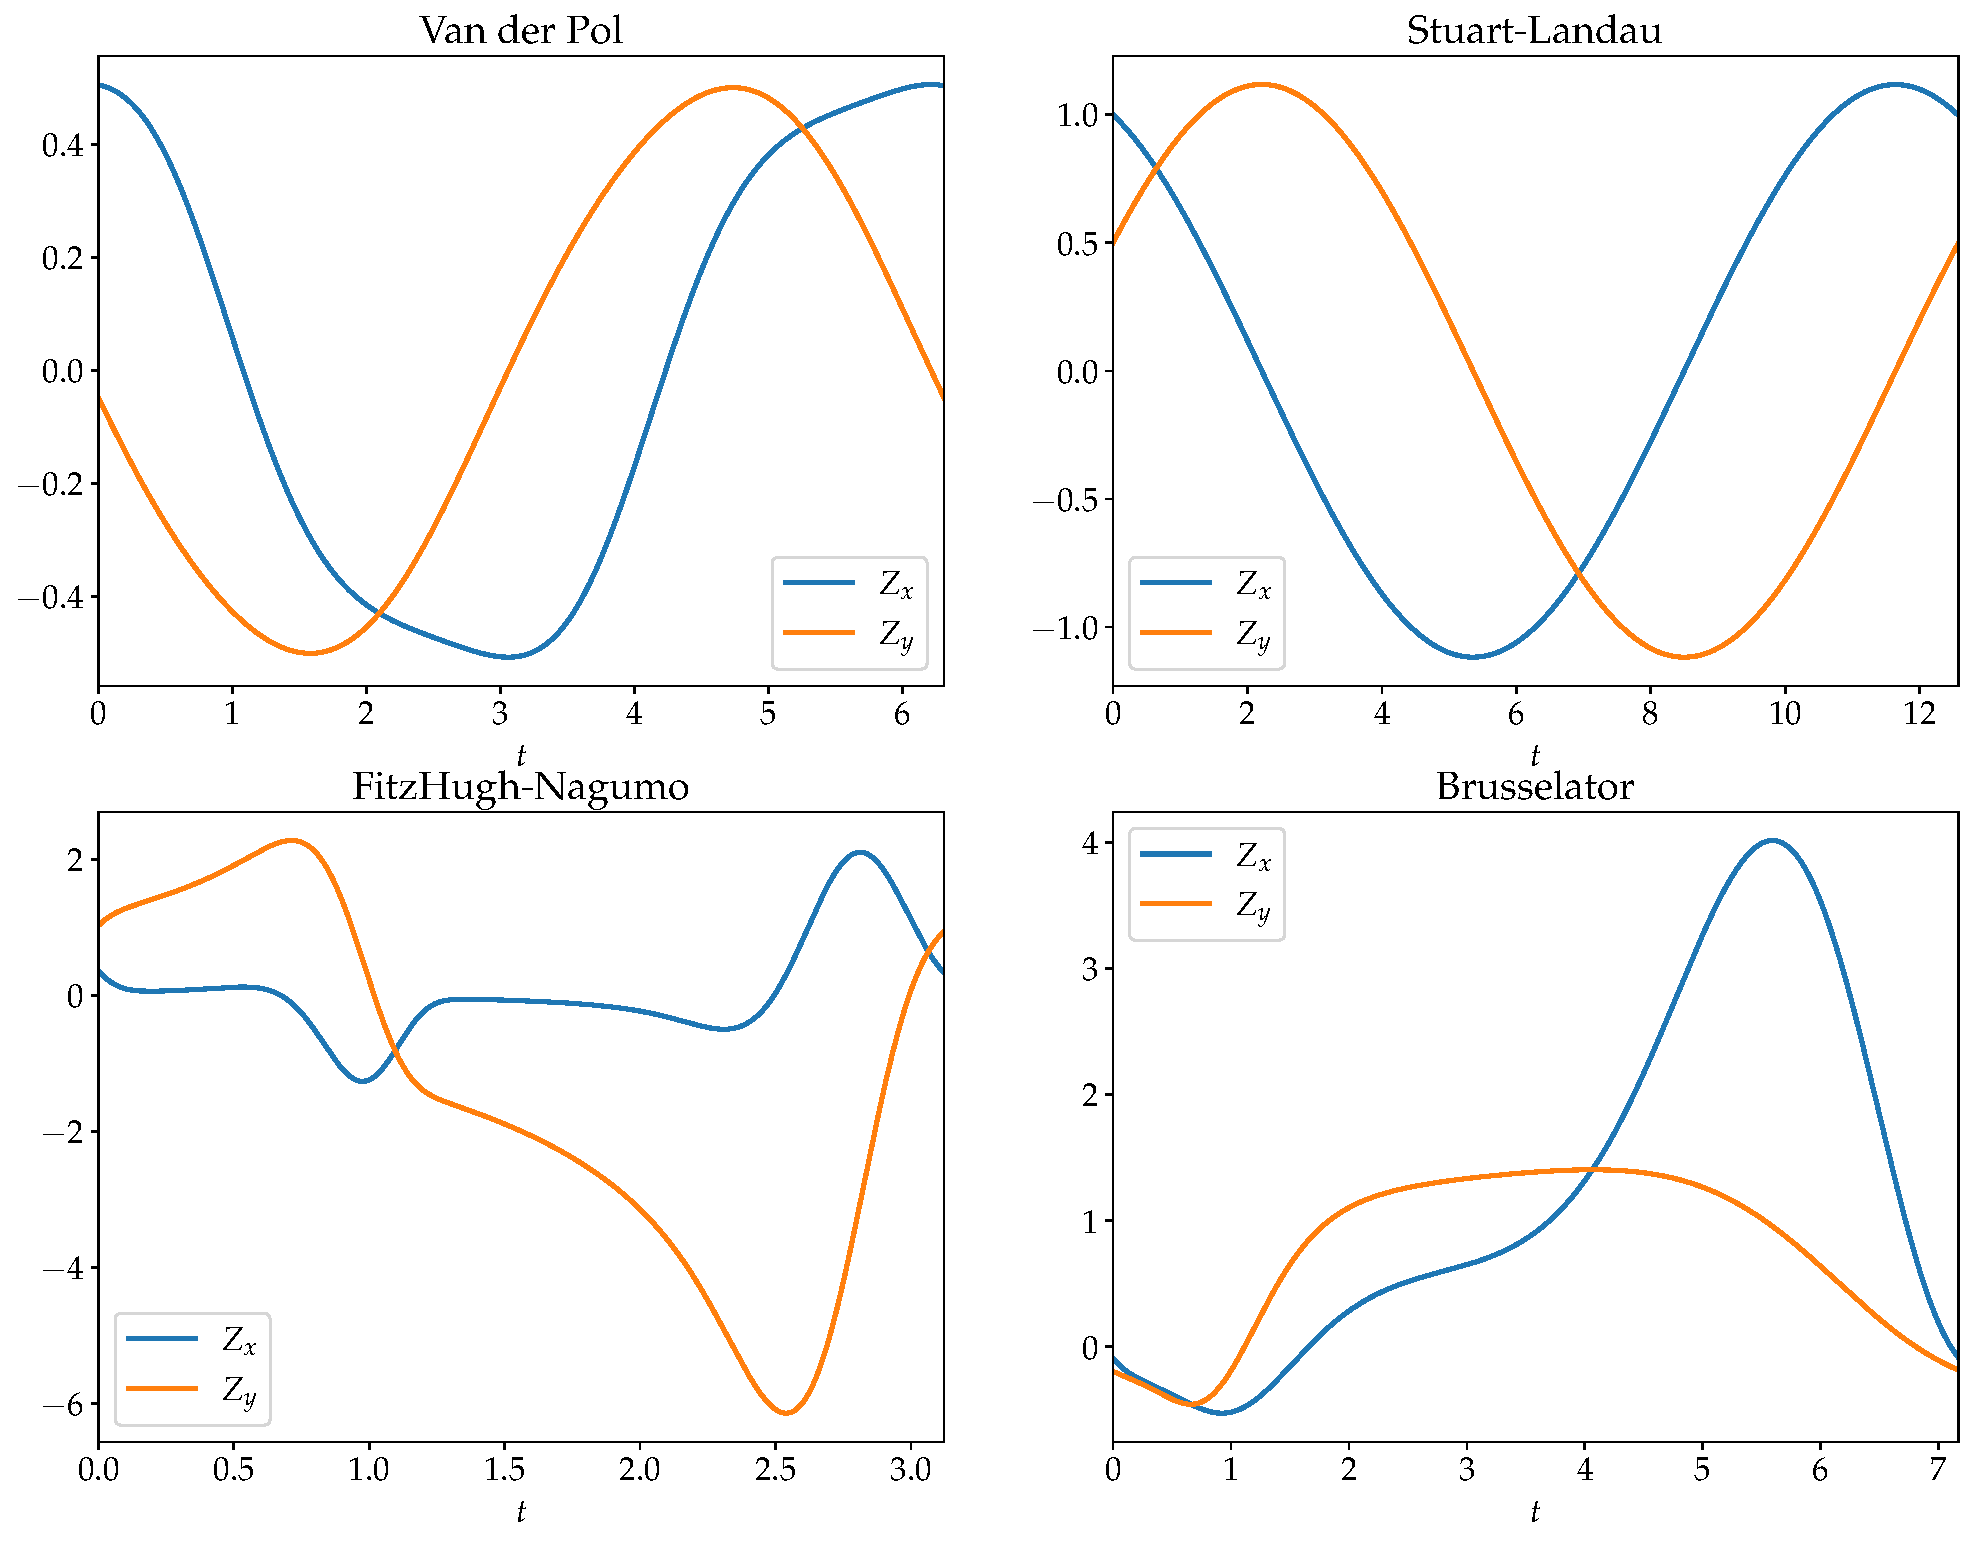
\includegraphics[width=0.8\textwidth]{figs/prc.pdf}
  \caption{Phase response curves for several ODEs having a stable periodic orbit.}
  \label{fig:prc}
\end{figure}

The same procedure can be applied to the case of coupled systems.
For example, let us consider the following $N$-body system:
\begin{align}
  \frac{\diff x_{i}}{\diff t}=f(x_{i})+\varepsilon f_{i}(x)+\varepsilon\sum_{j=1}^{N} g_{ij}(x_{i},x_{j}),\quad i=1,2,\dots,N,
  \label{eq:ode-coupled}
\end{align}
where $f_{i}\colon\mathbb{R}^{d}\to\mathbb{R}^{d}$ and $g_{ij}\colon\mathbb{R}^{d}\times\mathbb{R}^{d}\to\mathbb{R}^{d}$ are perturbation functions.
The unperturbed version of this equation $\dot{x}_{i}=f(x_{i})$ has a stable periodic orbit homeomorphic to $N$-dimensional torus $\mathbb{T}^{d}$.
Applying the same procedure as the previous subsection, we have the phase equation of \eqref{eq:ode-coupled} as
\begin{align}
  \frac{\diff\phi_{i}}{\diff t}=\omega_{i}+\varepsilon Z(\phi_{i})\left(F_{i}(\phi_{i})+\sum_{j=1}^{N}G_{ij}(\phi_{i},\phi_{j})\right),\quad i=1,2,\dots,N,
  \label{eq:perturbed-phase-diff-coupled}
\end{align}
where $F_{i}(\phi_{i})=f_{i}(p(\phi_{i}/\omega))$ and $G_{ij}(\phi_{i},\phi_{j})=g_{ij}(p(\phi_{i}/\omega),p(\phi_{j}/\omega))$.

\subsection{Method of averaging}
Basically the phase equatuion is derived in the previous subsection, but we can further make the equation simpler by the \textbf{method of averaging}.

We first consider the equation \eqref{eq:perturbed-phase-diff} with $G(t,\phi)=G(\phi)$.
By denoting $S(\phi)=Z(\phi)G(\phi)$, we have the following equation:
\begin{align}
  \dot{\phi}=\omega + \varepsilon S(\phi).
  \label{eq:perturbed-phase-diff-1}
\end{align}
By integrating both sides with respect to time, we have
\begin{align}
  \phi(t+\tau)-\phi(t)=\omega\tau+\varepsilon\int_{t}^{t+\tau}S(\phi(t+t'))\diff t'=\omega\tau+\mathcal{O}(\varepsilon T).
\end{align}
Here we make a bold assumption that we can rewrite $\dot{\phi}$ with a averaged velocity $\langle\dot{\phi}\rangle\coloneqq(1/T)\int_{t}^{t+T}\dot{\phi}(\tau)\diff\tau$\footnote{It turns out that this assumption is justified via the \textbf{near-identity transformation}, but we do not discuss it here.}.
Then we can expand the equation \eqref{eq:perturbed-phase-diff-1} with respect to $\varepsilon$:
\begin{align}
  \dot{\phi}\thickapprox \omega+\frac{\varepsilon}{T}\int_{0}^{T}S(\phi(t)+\omega t'+\mathcal{O}(\varepsilon T))\diff t'=\omega+\varepsilon\omega_{1}+\mathcal{O}(\varepsilon^{2}T),
\end{align}
where
\begin{align}
  \omega_{1}\coloneqq\frac{1}{2\pi}\int_{0}^{2\pi}S(\eta)\diff\eta.
\end{align}
This is the phase equation and the angle velocity becomes $\omega+\varepsilon\omega_{1}$.

For the case of coupled systems, we obtained the phase equation \eqref{eq:perturbed-phase-diff-coupled} in the previous subsection.
By averaging the equation with respect to time similar to the above paragraph,
we have the following equation:
\begin{align}
  \dot{\phi}_{i}=\omega+\varepsilon\omega_{i}+\varepsilon\sum_{j=1}^{N}\Gamma_{ij}(\phi_{i}-\phi_{j}),
  \label{eq:perturbed-phase-diff-coupled-1}
\end{align}
where the coupling function $\Gamma_{ij}(\phi)$ is calculated by
\begin{align}
  \Gamma_{ij}(\phi)\coloneqq\frac{1}{2\pi}\int_{0}^{2\pi}Z(\phi+\eta)G_{ij}(\phi+\eta,\phi)\diff\eta.
\end{align}
By the method of averaging, the phase equation \eqref{eq:perturbed-phase-diff-coupled-1} now becomes shift-invariant, that is the vector field is invariant under the shift $\phi_{i}\mapsto\phi_{i}+c$ for all $i$, which makes the analysis much easier than the original equation \eqref{eq:ode-coupled}.

\section{Coupled phase-oscillator models}
\label{sec:review-cpo}

In the previous section, we have derived the phase equation of the coupled ODEs in the form of \eqref{eq:perturbed-phase-diff-coupled-1}.
We can rewirte the equation in the general form as follows:
\begin{align}
  \frac{\diff\theta_{i}}{\diff t}=\omega_{i}+\sum_{j=1}^{N}\Gamma_{ij}(\phi_{i}-\phi_{j}),
  \label{eq:coupled-phase-oscillator}
\end{align}
and we call this equation the \textbf{coupled phase-oscillator model}.
In this section, we review the theoretical results of the coupled phase-oscillator models, especially focusing on the \textbf{Kuramoto model}.

\subsection{The Kuramoto model}
The Kuramoto model consists of $N$ phase-oscillators where $N$ is a large integer,
and evolutes in time with the following equations,
\begin{align}
  \frac{\diff\theta_{i}}{\diff t}=\omega_{i}+\frac{K}{N}\sum_{j=1}^{N}\sin(\theta_{j}-\theta_{i}),
  \label{eq:kuramoto-N}
\end{align}
for $i=1,\dots,N$.
$\theta_{i},~\omega_{i}$ are the phase and the natural frequency 
of the $i$th oscillator,
and each $\omega_{i}$ is drawn from a distribution $g(\omega)$,
which we call the natural frequency distribution.
In this thesis, we assume that $g(\omega)$ is symmetric and unimodal,
or more precisely,
$g(-\omega)=g(\omega)$ and $g'(\omega)<0$ for $\omega>0$.
Each oscillator is coupled through the sine function of the phase difference
with a homogeneous coupling strength $K\geq 0$.
When we take $K=0$,
there are no interactions among oscillators,
and they move with their own frequencies $\omega_{i}$,
On the other hand, when $K>0$ is sufficiently large,
oscillators tend to attract each other,
as we discuss later.

To visualize the extent of synchronization of oscillators,
the complex order parameter $z$ is introduced,
\begin{align}
  z=re^{i\phi}=\frac{1}{N}\sum_{j=1}^{N}e^{i\theta_{j}},
\end{align}
where $r,\phi\in\mathbb{R}$.
This order parameter $z$ represents the centroid of the oscillators
moving on the complex unit circle $\mathbb{S}^{1}$.
\begin{figure}[htb]
  \begin{center}
    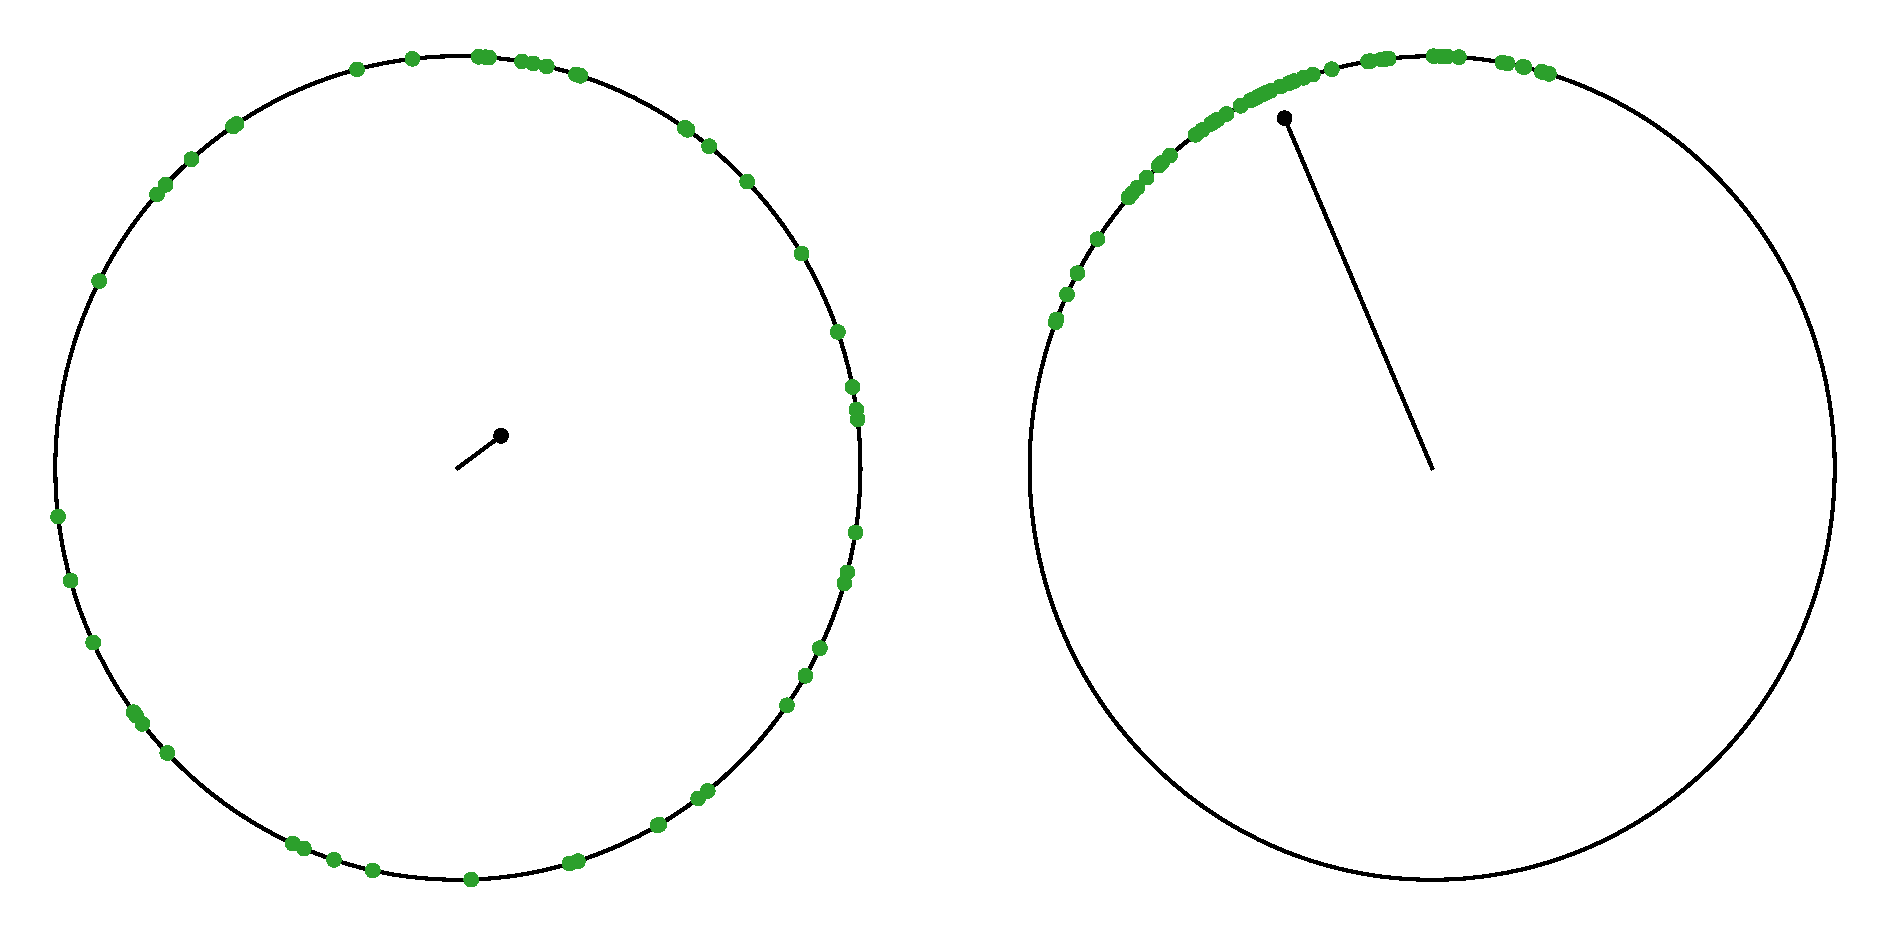
\includegraphics[width=14cm]{figs/order_disorder.pdf}
    \caption{Oscillators moving on $\mathbb{S}^{1}$.
    When the oscillators are uniformly distributed on $\mathbb{S}^{1}$,
    the centroid is close to $0$ (left).
    When the oscillators gather around a point on $\mathbb{S}^{1}$,
    $r$ gets close to $1$ (right).
    }
    \label{fig:circle}
  \end{center}
\end{figure}
%\begin{figure}[htb]
%  \begin{center}
%  \begin{tikzpicture}[line cap=round,line join=round,>=triangle 45,x=1.0cm,y=1.0cm]
%  \clip(-4.1,-0.58) rectangle (7.02,4.74);
%  \draw(-1,2) circle (2cm);
%  \draw(4,2) circle (2cm);
%  \draw[<-] (3.76,3.06)-- (4,2);
%  \draw (3.84,3.16) node[anchor=north west] {$z$};
%  \begin{scriptsize}
%  \fill [color=black] (-1,2) circle (2.0pt);
%  \fill [color=black] (4,2) circle (2.0pt);
%  \fill [color=black] (-2.02,3.72) circle (2.0pt);
%  \fill [color=black] (-2.78,2.9) circle (2.0pt);
%  \fill [color=black] (-0.11,3.79) circle (2.0pt);
%  \fill [color=black] (0.96,2.42) circle (2.0pt);
%  \fill [color=black] (0.64,0.85) circle (2.0pt);
%  \fill [color=black] (-2.5,0.68) circle (2.0pt);
%  \fill [color=black] (-2.97,1.68) circle (2.0pt);
%  \fill [color=black] (-0.9,0) circle (2.0pt);
%  \fill [color=black] (0.02,0.28) circle (2.0pt);
%  \fill [color=black] (-0.8,3.99) circle (2.0pt);
%  \fill [color=black] (0.98,1.72) circle (2.0pt);
%  \fill [color=black] (3.49,3.93) circle (2.0pt);
%  \fill [color=black] (3.04,3.76) circle (2.0pt);
%  \fill [color=black] (2.74,3.55) circle (2.0pt);
%  \fill [color=black] (4.1,4) circle (2.0pt);
%  \fill [color=black] (3.83,3.99) circle (2.0pt);
%  \fill [color=black] (2.48,3.3) circle (2.0pt);
%  \fill [color=black] (4.44,3.95) circle (2.0pt);
%  %\fill [color=black] (3.76,3.06) circle (2.0pt);
%  \end{scriptsize}
%  \end{tikzpicture}
%  \caption{Oscillators moving on $\mathbb{S}^{1}$.
%  When the oscillators are uniformly distributed on $\mathbb{S}^{1}$,
%  the centroid is close to $0$ (left).
%  When the oscillators gather around a point on $\mathbb{S}^{1}$,
%  $r$ gets close to $1$ (right).
%  }
%  \label{fig:circle}
%  \end{center}
%\end{figure}
As shown in Fig.~\ref{fig:circle},
when the oscillators are uniformly distributed on $\mathbb{S}^{1}$,
which corresponds to the nonsynchronized state,
$r$ gets close to $0$.
On the other hand,
when the oscillators gather at a point on $\mathbb{S}^{1}$,
which corresponds to the synchronized state, $r$ equals $1$.
Calculating $r$ is therefore useful for monitoring synchronization of the Kuramoto model.
We will look into the relation between the order parameter $r$
and the coupling strength $K$.

We give a brief explanation why the Kuramoto model describes synchronization.
Using the order parameter,
the equations of the Kuramoto model are written as
\begin{align}
  \frac{\diff\theta_{i}}{\diff t}=\omega_{i}+Kr\sin(\phi-\theta_{i}).
  \label{eq:kuramoto-orderparameter}
\end{align}
In the previous equations (\ref{eq:kuramoto-N}),
each oscillator couples with the other oscillators,
but this modification allows us to treat each oscillator
as it couples only with the order parameter.
%\red{This} corresponds to the mean-field approximation,
%famously done in the statistical mechanics model.
%As we have stated above, each oscillator moves independently on $\mathbb{S}^{1}$
%when the coupling strength $K=0$.
We will see what happens when $K$ is sufficiently large.
Let us assume that the phase of the $i$th oscillator is going ahead of the phase of the order parameter.
In this case $\sin(\phi-\theta_{i})$ is negative and this makes the $i$th phase $\theta_{i}$ slow down.
We can interpret this deceleration of the $i$th phase as the $i$th oscillator being attracted to the order parameter.
When the order parameter is going ahead of the $i$th oscillator,
the deceleration changes to the acceleration and the $i$th oscillator gets attracted to the order parameter.

%In the later discussions,
%\begin{align}
%  \frac{\diff\theta_{i}}{\diff t}=\omega_{i}-Kr\sin\theta_{i}
%  \label{eq:kuramoto-orderparameter-smiple}
%\end{align}
%is used instead of (\ref{eq:kuramoto-orderparameter}) for the simplicity of calculations.
%(\ref{eq:kuramoto-orderparameter-smiple}) can be obtained
%just by shifting every phases $\theta_{i}\to\theta_{i}-\phi$ in (\ref{eq:kuramoto-orderparameter}).
%This corresponds to taking $\phi$ to zero.

\subsection{The synchronization transition}
The Kuramoto model is known to exhibit the synchronization transition
from the nonsynchronized state to (partially) synchronized states,
and the order parameter $r$ shows a continuous transition
\begin{align}
  r\propto(K-K_{\mathrm{c}})^{\beta}
\end{align}
around the critical point $K\gtrsim K_{\mathrm{c}}$,
where $\beta$ is the critical exponent.
We will look back to the original Kuramoto's analysis
and derive the self-consistent equation of $r$.
Also, we will review a discussion on the stability of the solution to the Kuramoto model.

In the large population limit $N\to\infty$,
by the conservation of the number of oscillators,
(\ref{eq:kuramoto-N}) can be written in the equation of continuity~\cite{lancellotti2004},
\begin{align}
  &\frac{\partial F}{\partial t}+\frac{\partial}{\partial\theta}(v[F]F)=0,\label{eq:eq-cont}\\
  &v[F]=\omega+K\int_{\mathbb{S}^{1}}\diff\theta'\int_{\mathbb{R}}\diff\omega'\sin(\theta'-\theta)F(\theta',\omega',t)\label{eq:vector-field},
\end{align}
where $F(\theta,\omega,t)$ is the probability distribution function
of $\theta$ and $\omega$ at the time $t$.
In other words, $F(\theta,\omega,t)\diff\theta\diff\omega$
represents the fraction of oscillators having phases
between $\theta$ and $\theta+\diff\theta$
and natural frequencies between $\omega$ and $\omega+\diff\omega$ at the time $t$.
From the normalization condition $\int_{\mathbb{S}^{1}}\diff\theta\int_{\mathbb{R}}\diff\omega F(\theta,\omega,t)=1$,
\begin{align}
  \int_{\mathbb{S}^{1}}\diff\theta F(\theta,\omega,t)=g(\omega).
  \label{eq:normal}
\end{align}
In this limit the order parameter is expressed by
\begin{align}
  z=re^{i\phi}=\int_{\mathbb{S}^{1}}\diff\theta\int_{\mathbb{R}}\diff\omega F(\theta,\omega,t)e^{i\theta}.
\end{align}
%By using the order parameter,
%\begin{align}
%  v[F]=\omega+Kr\sin(\phi-\theta)
%\end{align}

We first seek for a solution to (\ref{eq:eq-cont})
where oscillators distributed uniformly on $\mathbb{S}^{1}$.
In this case the distribution function has to be constant with respect to $\theta$.
From the normalization condition (\ref{eq:normal}),
%(\ref{eq:eq-cont}) has the uniform solution
the flat distribution is expressed by
\begin{align}
  f^{0}(\omega)=\frac{g(\omega)}{2\pi}.
\end{align}
Since this uniform solution $f^{0}(\omega)$ is independent of $K$,
\begin{align}
  z=\int_{\mathbb{S}^{1}}\diff\theta\int_{\mathbb{R}}\diff\omega f^{0}(\omega)e^{i\theta}=0  
\end{align}
is valid for all $K$.
This fact induces $v[f^{0}]=\omega$
and $f^{0}$ is a stationary solution of (\ref{eq:eq-cont})
as $\frac{\partial}{\partial\theta}(v[f^{0}]f^{0})=0$.

The stability analysis of $f^{0}(\omega)$ is studied
through the linearized equation around $f^{0}(\omega)$
by expanding (\ref{eq:eq-cont}) with $F=f^{0}+f$, which reads
\begin{align}
  \frac{\partial f}{\partial t}=\mathcal{L}f\coloneqq-\omega\frac{\partial f}{\partial\theta}-Kf^{0}\Im(ze^{-i\theta}).
\end{align}
Here, $z$ reads
\begin{align}
  z=\int_{\mathbb{S}^{1}}\diff\theta\int_{\mathbb{R}}\diff\omega(f^{0}+f)e^{i\theta}=\int_{\mathbb{S}^{1}}\diff\theta\int_{\mathbb{R}}\diff\omega fe^{i\theta}.
\end{align}
$\mathcal{L}$ has a continuous spectrum on the imaginary axis.
This continuous spectrum was a huge obstacle to study the asymptotic behavior of the solution to the Kuramoto model,
but the generalized spectrum theory introduced by Chiba~\cite{chiba2015} solved this difficulty,
and the stability of $f^{0}(\omega)$ is solved;
for $K<K_{\mathrm{c}}\coloneqq2/(\pi g(0))$, $f^{0}(\omega)$ is asymptotically stable,
whereas unstable for $K>K_{\mathrm{c}}$.
%and Conjecture \ref{conj:kuramoto} was proved~\cite{chiba2015}.

%To seek for the limit of $F$ in the long time
To obtain the bifurcation diagram of the stationary solutions,
%for $K>K_{\mathrm{c}}$, where $f^{0}(\omega)$ is unstable,
%we derivate the self-consistency equation with respect to $r$.
we derivate the stationary solution of (\ref{eq:eq-cont}) for a given $K$.
%We shall assume that $F$ converges to the stationary state $F^{\mathrm{st}}(\theta,\omega)$,
%and we seek for $F^{\mathrm{st}}(\theta,\omega)$.
%We define the stationary state $F^{\mathrm{st}}(\theta,\omega)$ to satisfy
The stationary solution $F^{\mathrm{st}}(\theta,\omega)$ is defined so as to satisfy
\begin{align}
  \frac{\partial}{\partial\theta}(v[F^{\mathrm{st}}]F^{\mathrm{st}})=0,
  \label{eq:stationarity}
\end{align}
which implies $\frac{\partial}{\partial t}F^{\mathrm{st}}=0$.
This stationary solution $F^{\mathrm{st}}(\theta,\omega)$ gives a constant order parameter,
hence $r$ and $\phi$ are constant.
By shifting the frame with the phase $\phi$,
we can set $\phi$ to zero without loss of generality.
Then the velocity field becomes $v[F^{\mathrm{st}}]=\omega-Kr\sin\theta$.
The value of $r$ is unknown
because it is determined by $F^{\mathrm{st}}$, which we will compute in the following, as
\begin{align}
  r=\int_{\mathbb{S}^{1}}\diff\theta\int_{\mathbb{R}}\diff\omega\cos\theta F^{\mathrm{st}}(\theta,\omega).
\end{align}
We will determine the value of $r$ self-consistently.

The solution of (\ref{eq:stationarity}) is separately written in two parts of the $\omega$-axis.
An oscillator with $|\omega|<Kr$ has two fixed points of $\theta$ solving
\begin{align}
  v[F^{\mathrm{st}}]=\omega-Kr\sin\theta=0.
\end{align}
One solution is in the interval $|\theta|<\pi/2$
and the other is in $\pi/2<|\theta|<\pi$.
Looking back (\ref{eq:kuramoto-orderparameter}),
we observe that the derivation of $v$ is negative (positive)
at the former (latter) fixed point,
and hence it is stable (unstable).
All the oscillators having the natural frequency $\omega$ converge to the above stable fixed point,
therefore $F^{\mathrm{st}}\propto\delta(\omega-Kr\sin\theta)$.
From the normalization condition
\begin{align}
  \int_{-\pi/2}^{\pi/2}\diff\theta F^{\mathrm{st}}(\theta,\omega)=g(\omega),
\end{align}
the stationary solution is
\begin{eqnarray}
  F^{\mathrm{st}}_{\mathrm{lock}}(\theta,\omega)=\left\{
    \begin{array}{ll}
      \sqrt{(Kr)^{2}-\omega^{2}}\delta(\omega-Kr\sin\theta)g(\omega),&|\theta|<\frac{\pi}{2},\\
      0,&\frac{\pi}{2}<|\theta|<\pi.
  \label{eq:rho-lock}
    \end{array}
  \right.
\end{eqnarray}
We refer to these oscillators as the locked oscillators.
In contrast,
a oscillator with $|\omega|>Kr$ does not have fixed points,
and they drift on $\mathbb{S}^{1}$.
From the stationarity condition (\ref{eq:stationarity}) and the normalization condition (\ref{eq:normal}),
\begin{align}
  F_{\mathrm{drift}}^{\mathrm{st}}(\theta,\omega)=\frac{g(\omega)}{2\pi}\frac{\sqrt{\omega^{2}-(Kr)^{2}}}{|\omega-Kr\sin\theta|}.
  \label{eq:rho-drift}
\end{align}
We check the validity of \eqref{eq:rho-lock} and \eqref{eq:rho-drift} by numerical simulation.
We consider the Kuramoto model with $K=5.0$ and $N=50000$ oscillators and see the scattering plot with theoretical line $\omega=Kr\sin\theta$ in Fig.~\ref{fig:kuramoto-scatter}.
\begin{figure}[htbp]
  \centering
  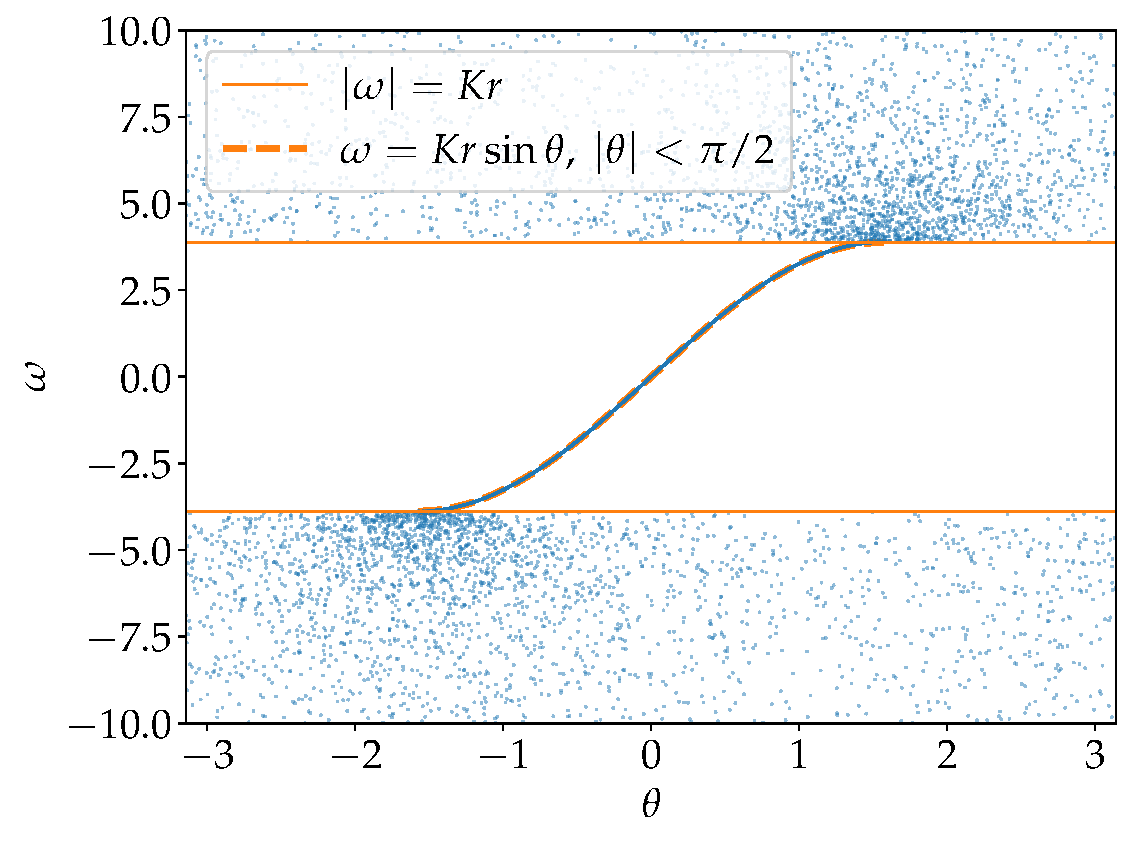
\includegraphics[width=0.7\textwidth]{figs/kuramoto_scatter.pdf}
  \caption{$(\theta,\omega)$ distribution of the Kuramoto model at $K=5.0$ with total number of oscillators $N=50000$.
  Numerical results are shown by scatter points and we see that the lock state is consisten with theoretical line $\omega=Kr\sin\theta$.}
  \label{fig:kuramoto-scatter}
\end{figure}

\eqref{eq:rho-lock} and \eqref{eq:rho-drift} depend on
unknown variable $r$,
and putting these two types of oscillators together,
we have the self-consistent equation for $r$ as
\begin{align}
  r=\int_{\mathbb{S}^{1}}\diff\theta\int_{|\omega|<Kr}\diff\omega\cos\theta F^{\mathrm{st}}_{\mathrm{lock}}(\theta,\omega)
  +\int_{\mathbb{S}^{1}}\diff\theta\int_{|\omega|>Kr}\diff\omega\cos\theta F^{\mathrm{st}}_{\mathrm{drift}}(\theta,\omega).
  \label{eq:self-consistent-original}
\end{align}
Since $F^{\mathrm{st}}_{\mathrm{drift}}(\theta+\pi,-\omega)=F^{\mathrm{st}}_{\mathrm{drift}}(\theta,\omega)$,
the contribution from the drifting oscillators cancels out,
and (\ref{eq:self-consistent-original}) is reduced to
\begin{align}
  r=Kr\int_{-\pi/2}^{\pi/2}\diff\theta\cos^{2}\theta g(Kr\sin\theta).
  \label{eq:self-consistency}
\end{align}
This equation has the trivial nonsynchronized solution $r=0$ for any $K$.
The (partially) synchronized solution $r\ne 0$ satisfies
\begin{align}
  1=K\int_{-\pi/2}^{\pi/2}\diff\theta\cos^{2}\theta g(Kr\sin\theta).
  \label{eq:self-consistency-divided}
\end{align}
Assuming that a partially synchronized branch bifurcates from $K=K_{\mathrm{c}}$,
we take the limit $K\to K_{\mathrm{c}}+0$ together with $r\to+0$
and we have the critical point
\begin{align}
  K_{\mathrm{c}}=\frac{2}{\pi g(0)},
  \label{eq:critical-point}
\end{align}
which is consistent with the value obtained from the stability analysis of $f^{0}(\omega)$.

When we set the natural frequency distribution $g(\omega)$ to Lorentzian distribution,
\begin{align}
  g(\omega)=\frac{\Delta}{\pi}\frac{1}{\omega^{2}+\Delta^{2}},
\end{align}
we can perform the integration in (\ref{eq:self-consistency}) and have
\begin{align}
  r=\sqrt{1-\frac{K_{\mathrm{c}}}{K}}
  \label{eq:r-lorentz}
\end{align}
for $K\geq K_{\mathrm{c}}=2\Delta$.
\begin{figure}[thbp]
  \begin{center}
    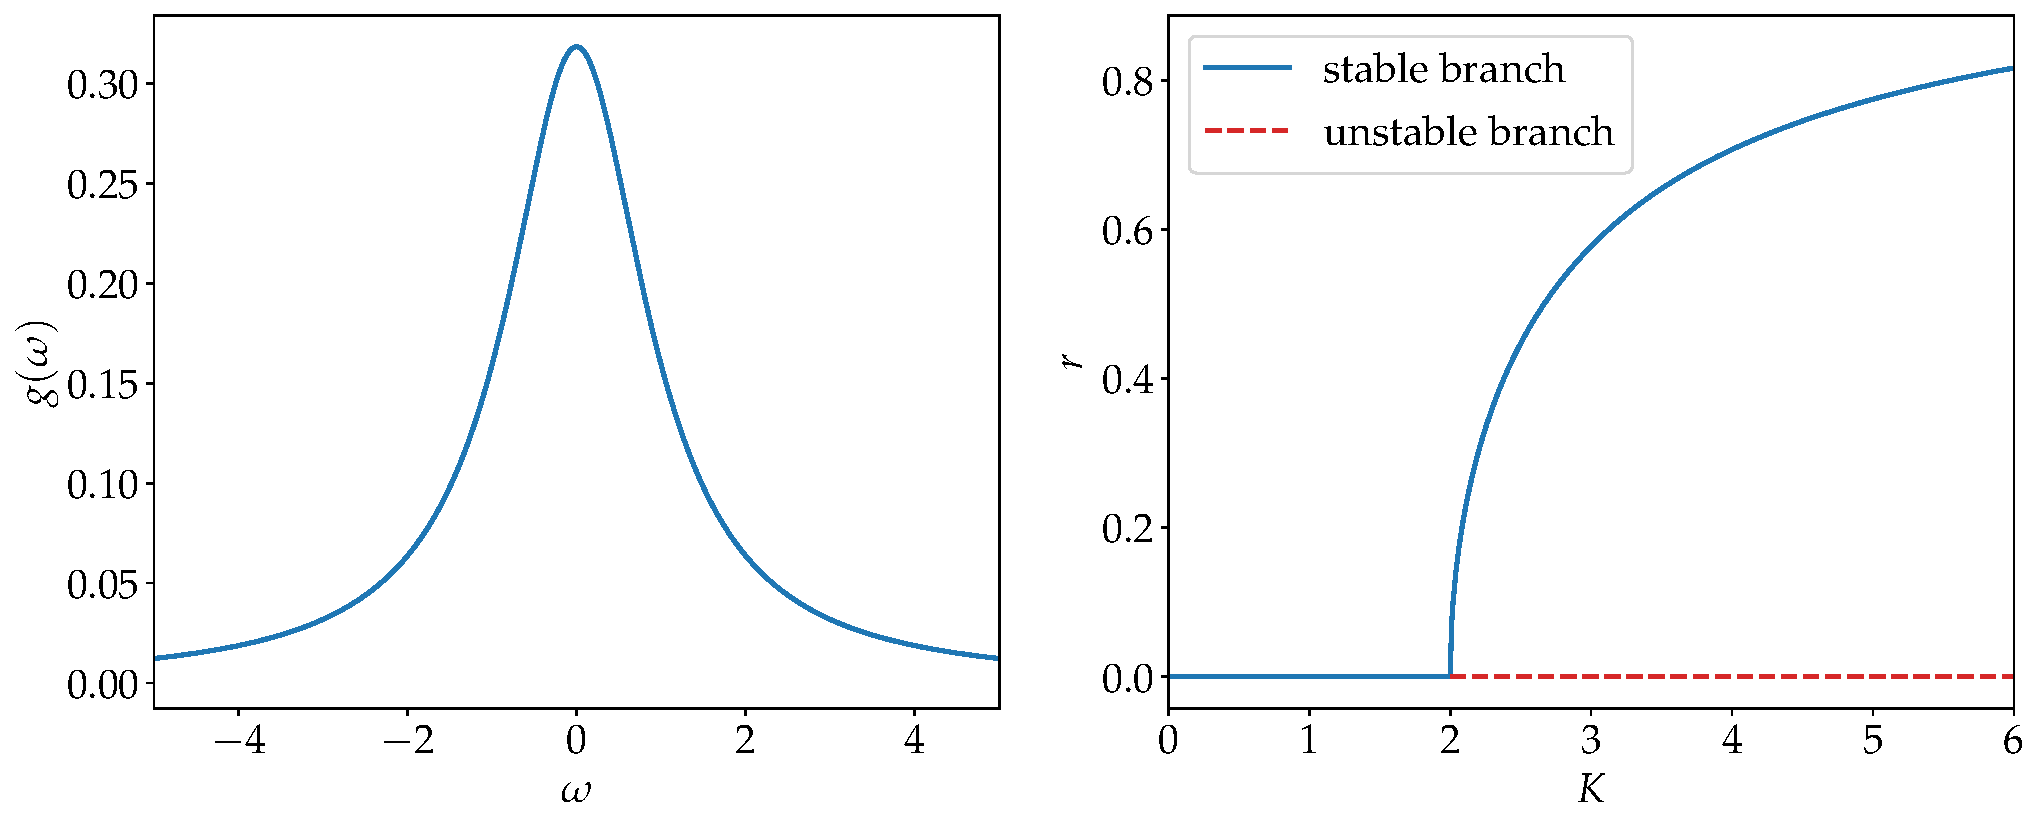
\includegraphics[width=\textwidth]{figs/lorentz-bif.pdf}
  \end{center}
  \caption{
    Lorentzian distribution (left) and the corresponding bifurcation diagram (right). We set $\Delta=1$.
    The stable/unstable branches are drawn in a solid/dashed line, respectively.
  }
  \label{fig:lorentz-bif}
\end{figure}
See Fig.~\ref{fig:lorentz-bif}.
Therefore, the partially synchronized branch bifurcates with $r\propto (K-K_{\mathrm{c}})^{1/2}$, and the critical exponent is $\beta=1/2$.
We will discuss the critical exponent for a general $g(\omega)$ in the next subsection.

%Based on this discussion,
%Kuramoto considered the following conjecture on the order parameter $r$ against the coupling constant $K$;
%\begin{conj}
%  \label{conj:kuramoto}
%  Suppose $N\to\infty$.
%  When $g(\omega)$ is symmetric and unimodal,
%  \begin{itemize}
%    \item $r=0$ is asymptotically stable for $K<K_{\mathrm{c}}$,
%    \item $r>0$ is asymptotically stable for $K>K_{\mathrm{c}}$,
%  \end{itemize}
%  where $K_{\mathrm{c}}:=2/(\pi g(0))$.
%\end{conj}

%The Kuramoto's analysis gives the exact stationary solutions of the Kuramoto model,
%but does not concern with stability of the solution.
%For the stability analysis,
%one has to consider the perturbation around a stationary solution.
%%(\ref{eq:eq-cont}) has the uniform solution
%%\begin{align}
%%  f^{0}(\omega)=\frac{g(\omega)}{2\pi},
%%\end{align}
%%which is corresponding to the nonsynchronized solution $r=0$,
%and the stability of $f^{0}(\omega)$ is studied
%through the linearized equation around $f^{0}(\omega)$
%by expanding (\ref{eq:eq-cont}) with $F=f^{0}+f$, which reads
%\begin{align}
%  \frac{\partial f}{\partial t}=\mathcal{L}f:=-\omega\frac{\partial f}{\partial\theta}-Kf^{0}\Im(ze^{-i\theta}).
%\end{align}
%Here, $z$ reads
%\begin{align}
%  z=\int_{\mathbb{S}^{1}}\diff\theta\int_{\mathbb{R}}\diff\omega(f^{0}+f)e^{i\theta}=\int_{\mathbb{S}^{1}}\diff\theta\int_{\mathbb{R}}\diff\omega fe^{i\theta}.
%\end{align}
%However, $\mathcal{L}$ has a continuous spectrum on the imaginary axis.
%This continuous spectrum was a huge obstacle to study the asymptotic behavior of the solution to the Kuramoto model,
%but the generalized spectrum theory introduced by Chiba solved this difficulty
%and Conjecture \ref{conj:kuramoto} was proved~\cite{chiba2015}.

We note on the unimodality and symmetry of the natural frequency distribution $g(\omega)$.
The above proof does not hold for $g(\omega)$ with bimodality or asymmetry,
which may yield different synchronization transitions~\cite{martens2009,terada2017,yoneda2019}.

%In this subsection we showed the Kuramoto's analysis,
%and we had the self-consistent equation (\ref{eq:self-consistency})
%for the order parameter $r$.
%We note that his analysis gives the exact solution,
%but does not concern with stability of the solution.
%For the stability analysis,
%one has to introduce the Kuramoto model in the large population limit $N\to\infty$.

\subsection{Critical exponents}
To calculate the critical exponent $\beta$ for general natural frequency distribution $g(\omega)$,
we expand (\ref{eq:self-consistency-divided}) around $r=0$, and we have
\begin{align}
  1=\frac{K}{K_{\mathrm{c}}}+\frac{K^{3}g''(0)}{16}r^{2}+\cdots.
\end{align}
Here, we used the critical point formula (\ref{eq:critical-point}).
However, this expansion is not enough when $g''(0)=0$,
and in this case we have to expand $g(\omega)$ up to higher degrees.
Therefore we assume that $g(\omega)$ has the following expansion around $\omega=0$,
\begin{align}
  g(\omega)=g_{n}(\omega)=g(0)-C_{n}\omega^{2n}+\cdots,
  \label{eq:g-n}
\end{align}
for $n\in\mathbb{N}$ where $C_{n}>0$, coming from the unimodality.
We set the second lower order of $g_{n}(\omega)$ to $2n$,
which is even because of the symmetry $g(-\omega)=g(\omega)$.
We note that the Lorentzian distribution and Gaussian distribution are
in the $n=1$ case.
We give two families of natural frequency distribution as examples of $g_{n}(\omega)$,
\begin{align}
  g^{(L)}_{n}(\omega)&=\frac{n\sin(\frac{\pi}{2n})}{\pi}\frac{\Delta^{2n-1}}{\omega^{2n}+\Delta^{2n}},\\
  g^{(G)}_{n}(\omega)&=\frac{n\Delta}{\Gamma(\frac{1}{2n})}e^{-\Delta^{2n}\omega^{2n}},
\end{align}
where $g^{(L)}_{n}(\omega)$ and $g^{(G)}_{n}(\omega)$ are generalizations
of the Lorentzian distribution and the Gaussian distribution, respectively~\cite{pietras2018}.
In the limit $n\to\infty$,
$g^{(L)}_{n}(\omega)$ and $g^{(G)}_{n}(\omega)$ converge to
\begin{align}
  g_{\infty}(\omega):
  =\begin{cases}
      \frac{1}{2\Delta},&\omega\in[-\Delta,\Delta],\\
      0,&\mathrm{otherwise}.
  \end{cases}
  \label{eq:g-infty}
\end{align}
This distribution is a uniform distribution on a compact support.
See Fig.~\ref{fig:yoko-dist}.
\begin{figure}[thbp]
  \begin{center}
    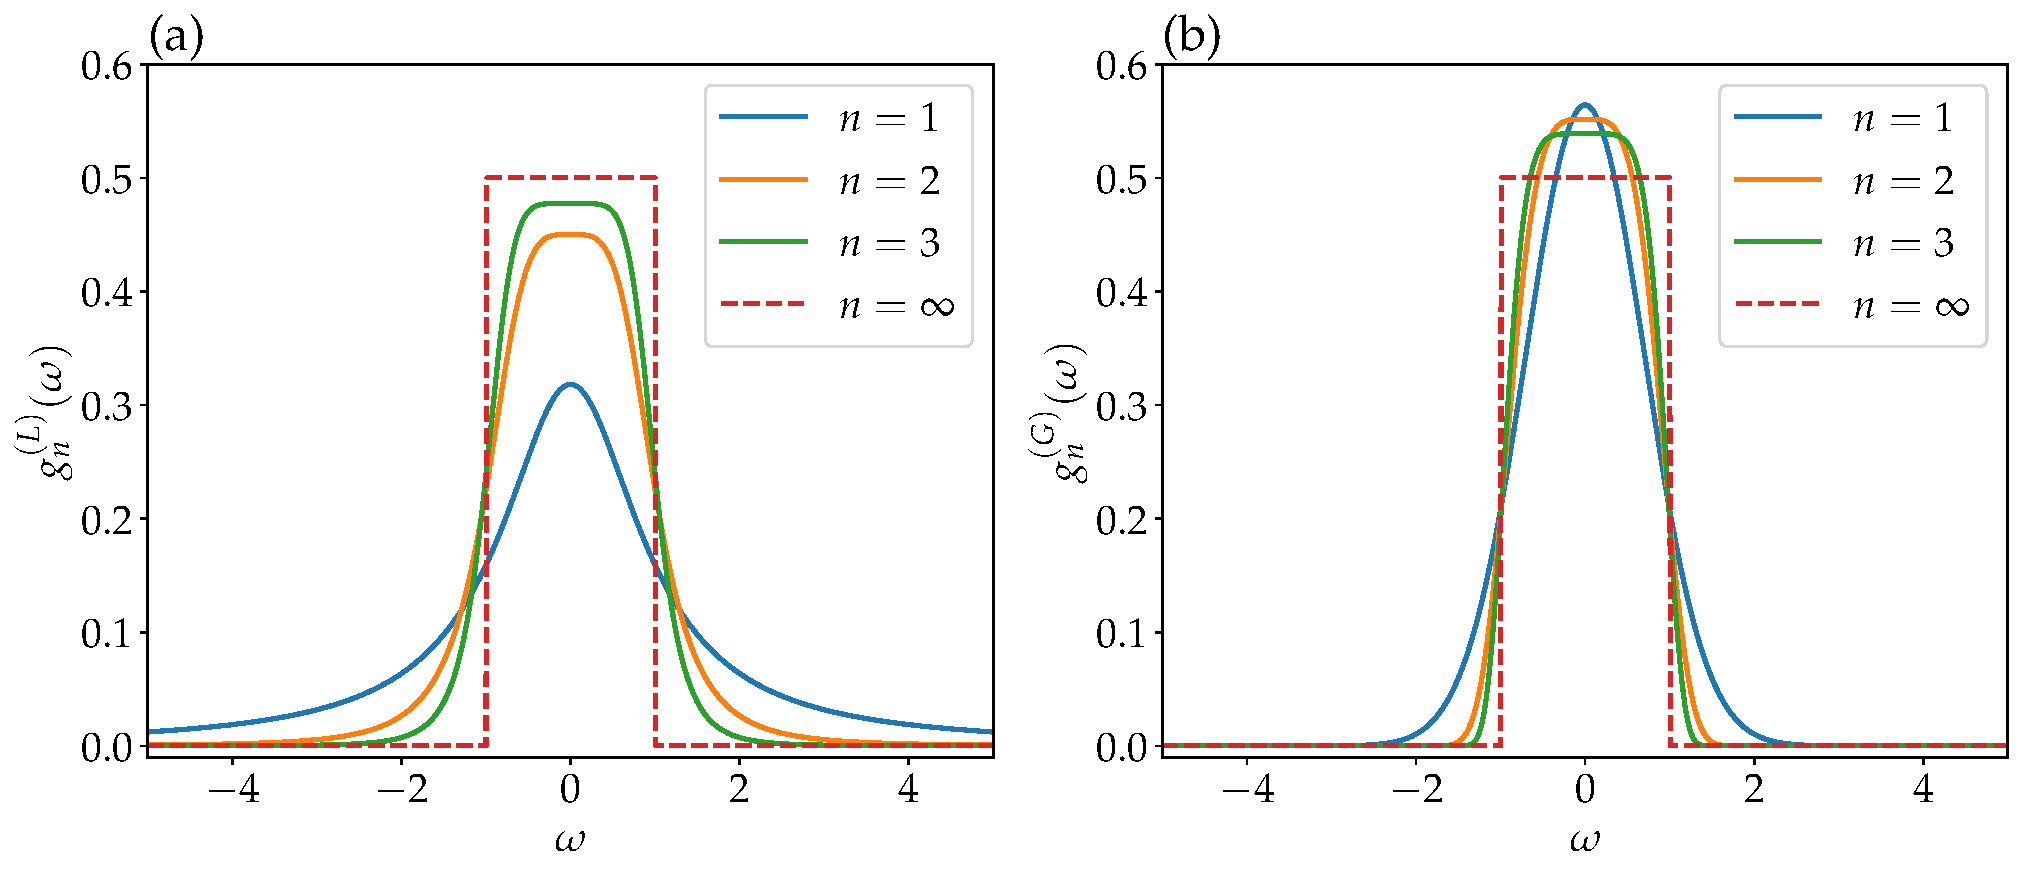
\includegraphics[width=\textwidth]{figs/general_dist.pdf}
  \end{center}
  \caption{
    Graphs of natural frequency distributions (a) $g^{(L)}_{n}(\omega)$ and (b) $g^{(G)}_{n}(\omega)$
    for $n=1,2,3,$ and $\infty$ for $\Delta=1$.
    $g^{(L)}_{n}(\omega)$ and $g^{(G)}_{n}(\omega)$ converge to $g_{\infty}(\omega)$ (\ref{eq:g-infty}).
  }
  \label{fig:yoko-dist}
\end{figure}

Let us observe the value of $\beta$ takes
for the distribution $g_{n}(\omega)$ (\ref{eq:g-n}).
We again expand (\ref{eq:self-consistency-divided}) around $r=0$,
\begin{align}
  &1=\frac{K}{K_{\mathrm{c}}}-D_{n}r^{2n}+\cdots,\\
  &D_{n}=C_{n}K_{\mathrm{c}}^{2n+1}B\left(n+\frac{1}{2},\frac{3}{2}\right),
\end{align}
where $B(x,y)$ is the beta function\footnote{The beta function is defined by $B(x,y)=\int_{0}^{1}t^{x-1}(1-t)^{y-1}\diff t$ for $\Re(x)>0$ and $\Re(y)>0$.}.
Therefore $r$ bifurcates from $K=K_{\mathrm{c}}$ with
\begin{align}
  r\sim\left(\frac{K-K_{\mathrm{c}}}{D_{n}K_{\mathrm{c}}}\right)^{\frac{1}{2n}}\propto(K-K_{\mathrm{c}})^{\frac{1}{2n}},
  \label{eq:r-g-n}
\end{align}
and the critical exponent is $\beta=1/(2n)$.
For the Lorentzian distribution,
(\ref{eq:r-g-n}) is consistent with (\ref{eq:r-lorentz}) since $n=1$.

What left to calculate is the critical exponent $\beta$
for $g_{\infty}(\omega)$ (\ref{eq:g-n}).
In this case,
$g_{\infty}(\omega)$ is no longer an analytic function,
hence we have to solve this case separately.
$g_{\infty}(\omega)$ is an uniform distribution,
and the discontinuity at the boundary of the support leads
to the jump in the order parameter at the critical point.
Reference \cite{basnarkov2007} has showed that the critical point $K=K_{\mathrm{c}}$
and the jump point $r_{\mathrm{c}}$ at $K=K_{\mathrm{c}}$ read
\begin{align}
  K_{\mathrm{c}}=\frac{4\Delta}{\pi},\quad r_{\mathrm{c}}=\frac{\pi}{4},
\end{align}
and the $K$-dependency of the order parameter $r$ reads
\begin{align}
  r-r_{\mathrm{c}}\propto(K-K_{\mathrm{c}})^{\frac{2}{3}}.
\end{align}
We note that this jump is different from the one we see
when $g(\omega)$ is bimodal \cite{martens2009,terada2017,yoneda2019} in the sense that
the jump with the uniform distribution exhibits no hysteresis,
whereas the jump with the bimodal distribution exhibits hysteresis.
%We also note for latter convenience that
%the finite-size scaling of the Kuramoto model with (\ref{eq:g-infty})
%is discussed in Ref.~\cite{coletta2017}.

\begin{figure}[htbp]
  \centering
  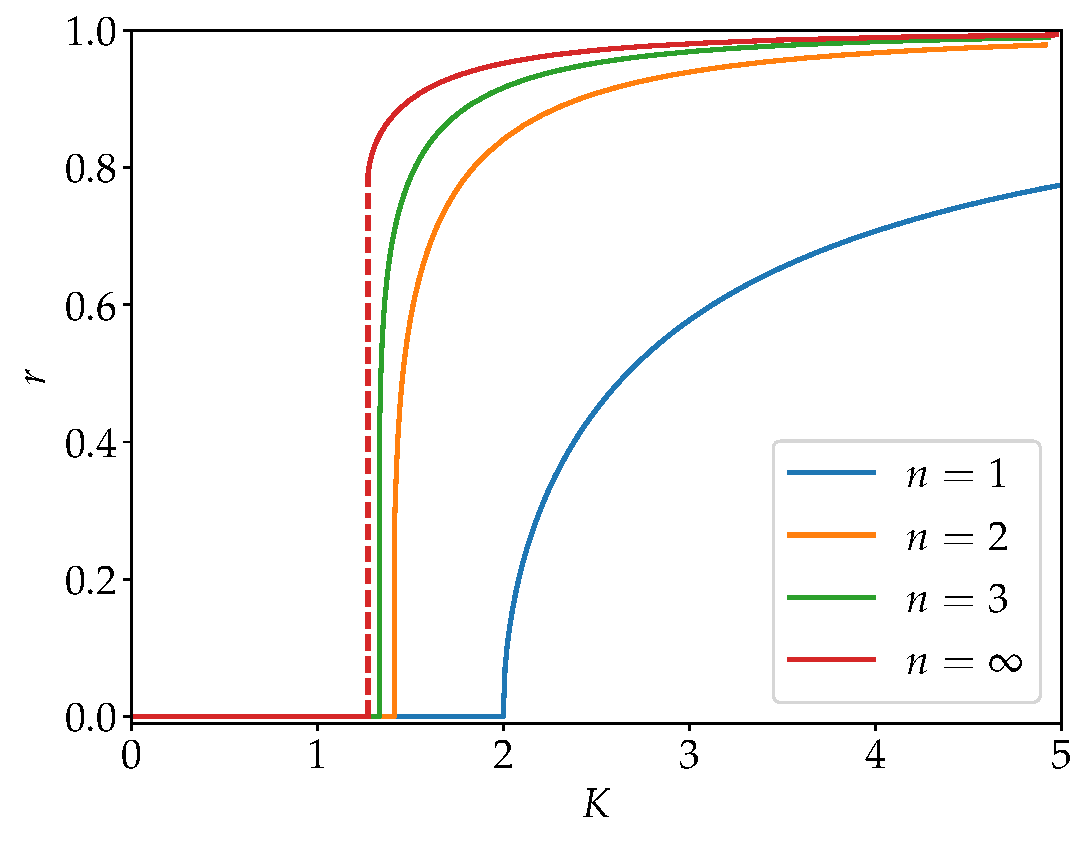
\includegraphics[width=0.7\textwidth]{figs/general_dist_bif_diagram.pdf}
  \caption{Stable branches of the Kuramoto model for natural frequency distributions $g_{n}^{(L)}(\omega)$ with $n=1,2,3,\infty$ for $\Delta=1$.}
  \label{fig:general_dist_bif_diagram}
\end{figure}

\subsection{General coupling functions}
%\red{OPTIONAL: MAYBE ADD EXPLANATION ON PHASE REDUCTION THEORY}
The Kuramoto model with a general coupled function is defined by
\begin{align}
  \frac{\diff\theta_{i}}{\diff t}=\omega_{i}+\frac{K}{N}\sum_{j=1}^{N}\Gamma(\theta_{j}-\theta_{i}),
  \label{eq:phase-oscillator}
\end{align}
where $\Gamma(\theta)$ is a $2\pi$-periodic function,
and the interactions depend on the phase difference $\theta_{j}-\theta_{i}$,
from the phase reduction theory~\cite{kuramoto2019}.
%Taking $\Gamma(\theta)=\sin\theta$,
%(\ref{eq:phase-oscillator}) falls back to the original Kuramoto model.

A natural and simple extension of the Kuramoto model is to add a bi-harmonic function~\cite{komarov2014}:
\begin{align}
  \Gamma(\theta)=\sin\theta+a\sin2\theta,\quad a<1.
  \label{eq:biharmonic}
\end{align}
When $a=0$, this model falls back to the original Kuramoto model (\ref{eq:kuramoto-N}).
Reference \cite{chiba2011} has proved that the order parameter exhibits a transcritical bifurcation
at the critical point $K=K_{\mathrm{c}}$ with
\begin{align}
  r\sim\frac{2(1-a)}{K_{\mathrm{c}}^{3}Ca}(K-K_{\mathrm{c}})\propto K-K_{\mathrm{c}},
\end{align}
where
\begin{align}
  C=\mathcal{PV}\int_{\mathbb{R}}\diff\omega\frac{g'(\omega)}{\omega}.
\end{align}
Here, $\mathcal{PV}$ represents the principal value of an integral.
$C$ takes a negative value for unimodal and symmetric $g(\omega)$.
Therefore, the critical exponent $\beta$ becomes unity when $a<0$
for unimodal and symmetric $g(\omega)$,
which is different from $\beta=1/(2n)$ in the Kuramoto model.
We note that this model exhibits a first-order phase transition when $0<a<1$
since $r<0$ is forbidden.
In Fig.~\ref{fig:kuramoto-biharmonic}, we show the numerical results of the Kuramoto model with (\ref{eq:biharmonic}).
We can see the hysteresis in the order parameter $r$ for $a=0.5$,
indicating the first-order phase transition.

\begin{figure}[htbp]
  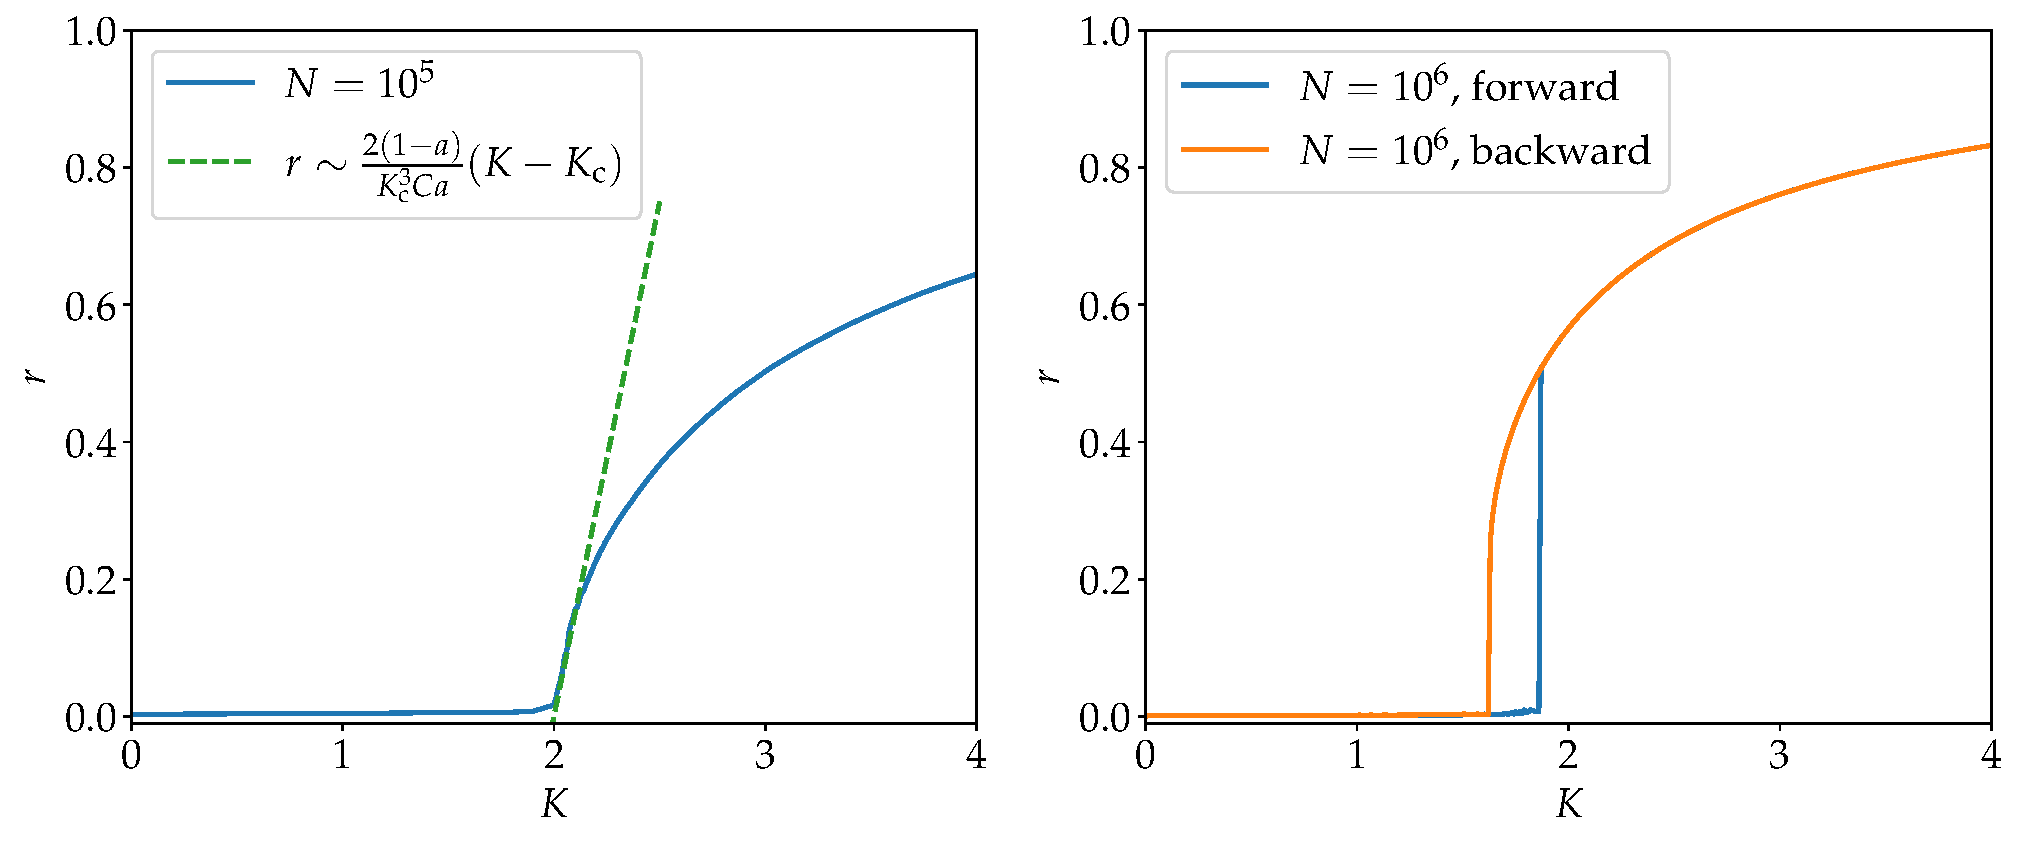
\includegraphics[width=\textwidth]{figs/kuramoto_biharmonic.pdf}
  \caption{Numerical results of the Kuramoto model with a bi-harmonic coupling function \eqref{eq:biharmonic} for $a=-0.2$ (left) and $a=0.5$ (right).
  }
  \label{fig:kuramoto-biharmonic}
\end{figure}

\subsection{Coupled phase-oscillator models on networks}
There exist many types of networks in the real-world,
such as human relationships, World Wide Web, citations of scientific papers, and so on.
We refer to these networks as complex networks,
and dynamical systems on the complex networks attract widespread interest.
See \cite{dorogovtsev2008} for a review of dynamical systems on complex networks,
especially on their critical phenomena.
The coupled phase-oscillator models are no exceptions,
and there are extensive researches on the coupled phase-oscillator models on complex networks.
One extended Kuramoto model on a complex network is
\begin{align}
  \frac{\diff\theta_{i}}{\diff t}=\omega_{i}+\frac{K}{\langle k\rangle}\sum_{j\in\Lambda_{i}}\sin(\theta_{j}-\theta_{i}),
  \label{eq:kuramoto-N-network}
\end{align}
for $i=1,\cdots,N$.
Here $\langle k\rangle$ is the average degree of the network,
and $\Lambda_{i}$ is the index set of the oscillators connecting to the $i$th oscillator.
If the network is all-to-all, $\langle k\rangle=N$ and $\Lambda_{i}=\{1,\cdots,N\}$,
therefore (\ref{eq:kuramoto-N-network}) falls back to the original Kuramoto model (\ref{eq:kuramoto-N}).
One of the most successful studies to tackle the model (\ref{eq:kuramoto-N-network}) is
to use a graphon~\cite{chiba2018},
defined by a symmetric measurable function $W:[0,1]^{2}\to[0,1]$,
which can be seen as, in some sense, a ``limit'' of the adjacency matrix of the network.
For an all-to-all network, the continuum limit graphon is $W(x,y)=1$ for all $x,y\in[0,1]$.
Another example is the Erd\H{o}s--R\'{e}nyi graph,
in which existence of an edge is probablistically determined with probability $p$,
and its graphon in the continuum limit is
\begin{align}
  W(x,y)=p,\quad \forall x,y\in[0,1].
\end{align}
There is only a constant difference between the all-to-all graph and the Erd\H{o}s--R\'{e}nyi graph,
therefore we can easily know the critical point and critical exponents of the Erd\H{o}s--R\'{e}nyi graph
from an analogy of previous discussions.

In \cite{chiba2018}, extended Kuramoto models on many other networks are discussed,
and their results suggest that the critical exponent are the same as the ones
in the all-to-all Kuramoto model.
Thus, we can see that graphons are a powerful tool to analyze the extended Kuramoto model on networks,
but we have to note that graphons can be defined only for a graph with $O(N^{2})$ edges
with $N$ nodes.
Whereas real-world networks are often very sparse, say $O(N)$ edges,
analyzing by graphons cannot be adopted to an extended Kuramoto model on a sparse network.
One of the most important networks with $O(N)$ edges is the small-world network.
In \cite{hong2002}, the critical exponent of the extended Kuramoto model on small-world networks
for the Gaussian distribution $g(\omega)$ is numerically calculated,
and it is claimed that $\beta=1/2$.
This value is the same as the one from the Kuramoto model with the Gaussian distribution,
but we do not know the dependency on natural frequency distributions $g(\omega)$
or coupling functions $\Gamma(\theta)$.
Moreover, in \cite{juhasz2019},
the critical exponent of the Kuramoto model on a sparse Erd\H{o}s--R\'{e}nyi network
for the Gaussian distribution is numerically calculated,
and it is claimed that $\beta=0.66$, which is different from $1/2$.
This result suggests that extended Kuramoto models on $O(N^{2})$ networks take the same critical exponent
as the Kuramoto model,
whereas extended Kuramoto models on $O(N)$ networks take different values.

In the next section,
we numerically calculate the critical exponent $\beta$ for coupled phase-oscillator models on small-world networks,
and observe dependence on $n$ of $g_{n}(\omega)$ or the coupling function $\Gamma(\theta)$
to reveal difference between the all-to-all network and the small-world network.
